
\begin{frame}
\frametitle{Klassifikation}

\begin{center}
\begin{tabular}{llll}
Klasse&Bedingung&Beispiel&Anwendung\\
\hline
elliptisch &$\begin{aligned}P&=n\mathstrut\end{aligned}$
	&$\displaystyle \Delta u=f                                $
		&Potential\\
&	&	&Eigenwertproblem\\
\hline
parabolisch&%$P=n-1, Z=1$
$\begin{aligned}P&=n-1\mathstrut\\Z&=1\mathstrut\end{aligned}$
	&$\displaystyle \frac{\partial u}{\partial t}=\Delta u    $
		&W"armeleitung\\
\hline
hyperbolisch&%$P=n-1, N=1$
$\begin{aligned}P&=n-1\mathstrut\\N&=1\mathstrut\end{aligned}$
	&$\displaystyle \frac{\partial^2 u}{\partial t^2}=\Delta u$
		&Wellen\\
\hline
\end{tabular}
\end{center}

Klasse verr"at:
\begin{itemize}
\item Charakter der L"osung: Schwingungen, exponentielles Abklingen
\item Welches L"osungsverfahren geeignet ist
\end{itemize}

\end{frame}

\begin{frame}
\frametitle{Problem}
Differentialgleichung
\begin{alignat}{2}
L u&=f\qquad&&\text{in $\Omega$}
\notag
\intertext{Randbedingungen}
  u&=g\qquad&&\text{auf $\partial\Omega$}
\notag
\end{alignat}
\pause
Allgemeine L"osung:
\begin{align*}
u&=u_p+u_r + u_h
\end{align*}
mit
\begin{align*}
L u_p&=  f&L u_r&=0    &L u_h&=0\\
  u_p&=\;?&  u_r&=g-u_p&  u_h&=0
\end{align*}
\begin{enumerate}
\item L"osung existiert $\Leftrightarrow \exists u_p, u_r$  
\item Eindeutigkeit der L"osung: $u_h=0$
\end{enumerate}
\end{frame}

\begin{frame}
\frametitle{Maximumprinzip}

Sei $L$ ein elliptischer Operator.

\begin{theorem}
Wenn $u$ im Gebiet $\Omega$ eine L"osung von $Lu=0$ ist, dann hat
$u$ kein lokales Minimum oder Maximum im Inneren von $\Omega$.
\end{theorem}

\pause

\begin{theorem}
Wenn $\Omega$ ein beschr"anktes und zusammenh"angendes Gebiet ist, 
dann hat eine L"osung von $Lu=0$ ihr Maximum und Minimum auf
dem Rand $\partial \Omega$.
\end{theorem}

\pause

\begin{theorem}
Wenn $\Omega$ beschr"ankt und zusammenh"angend ist, dann ist die 
L"osung des Randwertproblems eindeutig, falls sie existiert.
\end{theorem}

\end{frame}

\begin{frame}
\frametitle{Mittelwerteigenschaft}

\begin{theorem}
Ist $u$ eine harmonische Funktion im Gebiet $\Omega$, dann hat $u$ die
Mittelwerteigenschaft:
\[
u(x)
=
\frac{1}{\operatorname{vol}(S_r(x))}
\int_{S_r(x)}u(\xi)\,d\xi,
\]
wobei $S_r(x)$ eine Kugel mit Radius $r$ um den Punkt $x$ ist, die ganz
in $\Omega$ enthalten ist.
\end{theorem}

{\bf Achtung:} Gilt nur f"ur den gew"ohnlichen Laplace-Operator

\end{frame}

\begin{frame}
\frametitle{Greensche Funktion}
{\bf Problem:}
\begin{align*}
y''(x)&=f(x) \qquad\text{f"ur $x \in (0,1)$}\\
y(0)&=a\\
y(1)&=b
\end{align*}
{\bf Idee:} Gibt es einen inversen Operator der zweiten Ableitung?
\pause
Sieht aus wie eine Matrix
\[
y = \Delta^{-1}f,
\qquad
y(x)=\int_0^1 K(x,\xi)f(\xi)\,d\xi
\]
\pause
{\bf L"osung:} der sog.~Greenschen Funktion $G$:
\[
y(x)=\underbrace{\int_0^1 G(x,\xi)f(\xi)\,d\xi}_{u_p}
+
\underbrace{a(1-x) + bx}_{u_r}
\]
\end{frame}

\begin{frame}
\frametitle{Greensche Funktion}
\begin{align*}
G(x,\xi)
&=
\begin{cases}
(x-\xi) + x(1-\xi) = \xi(x - 1)&\qquad x\ge \xi\\
x(\xi-1)&\qquad x<\xi
\end{cases}
\end{align*}
\includegraphics[width=\hsize]{../../skript/images/green-1.pdf}
\end{frame}

\begin{frame}
\frametitle{Greensche Funktion}
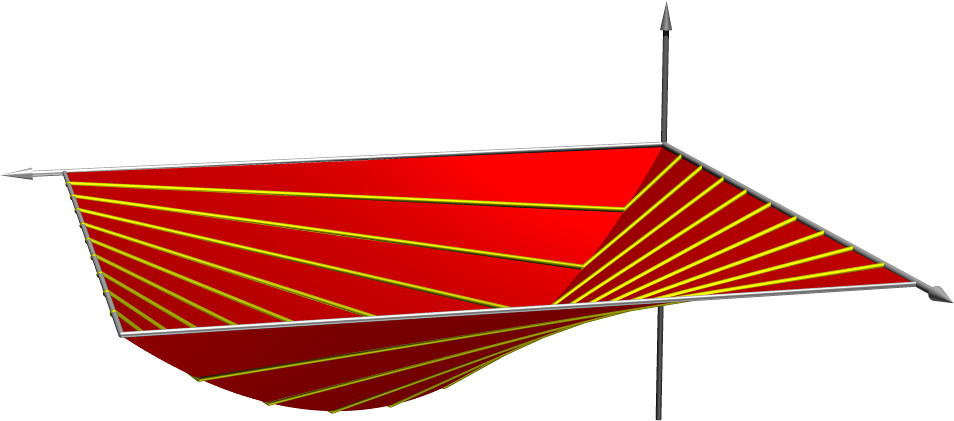
\includegraphics[width=\hsize]{../../skript/3d/green.jpg}
\end{frame}

\begin{frame}
\frametitle{Greensche Funktion}
\includegraphics[width=\hsize]{../../skript/graphics/green-1.pdf}
\end{frame}

\begin{frame}
\frametitle{Greensche Funktion}
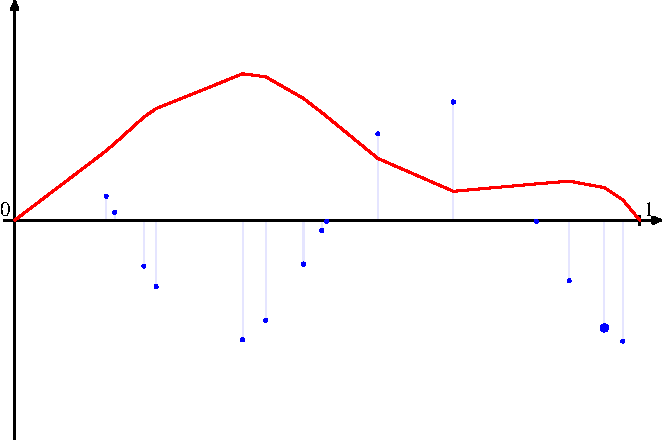
\includegraphics[width=\hsize]{../../skript/graphics/green-324.pdf}
\end{frame}

\begin{frame}
\frametitle{Greensche Funktion}
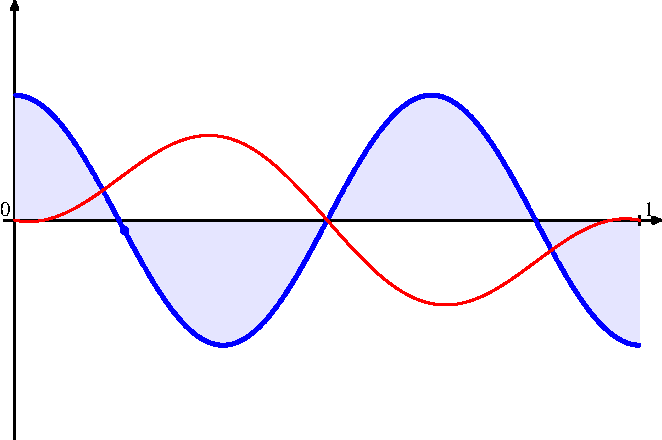
\includegraphics[width=\hsize]{../../skript/graphics/green-1082.pdf}
\end{frame}

\begin{frame}
\frametitle{Greensche Funktion, $n=1$}
Alternative Konstruktion der Greenschen Funktion
\begin{enumerate}[<+->]
\item Einheits-``Knick'':
\[
\sigma(x,\xi)=\frac12|x-\xi|\qquad\text{erf"ullt}\qquad \Delta\sigma(x,\xi)=\delta(x-\xi)
\]
\item ``harmonische'' Funktion $h(x,\xi)$ mit gleichen Randwerten:
\[
h(x,\xi)=(1-x)\sigma(0,\xi) + x\sigma(1,\xi)
\]
\item Greensche Funktion:
\[
G(x,\xi) = \sigma(x,\xi) - h(x,\xi)
\]
\end{enumerate}
\pause
Eigenschaften von $G$:
\begin{align*}
\Delta G(x,\xi)&=\delta(x-\xi)\\
G(0,\xi)&=\sigma(0,\xi)-(1-0)\sigma(0,\xi)+0\cdot\sigma(1,\xi)=0\\
G(1,\xi)&=\sigma(1,\xi)-0\cdot\sigma(1,\xi)-\sigma(1,\xi)=0
\end{align*}
\end{frame}

\begin{frame}
\frametitle{Greensche Funktion, $n>1$}
\begin{enumerate}[<+->]
\item
Einheits-``L"osung'':
\[
\sigma(x,\xi) = \begin{cases}
\displaystyle\frac1{2\pi}\log|x-\xi|\quad&n=2\\
\\
\displaystyle-\frac1{4\pi}\frac{1}{|x-\xi|}\quad&n=3
\end{cases}
\]
und weitere f"ur $n>3$
\item
$h(x,\xi)$ durch L"osung des Randwertproblems
\begin{align*}
\Delta h(x,\xi)&= 0\quad\text{in $\Omega$},&h(x,\xi)&=\sigma(x,\xi)\quad\text{auf $\partial\Omega$}
\end{align*}
f"ur jedes $\xi$
\item Greensche Funktion
\[
G(x,\xi)=\sigma(x,\xi)-h(x,\xi)
\]
\end{enumerate}
\end{frame}


\begin{frame}
\frametitle{Greensche Funktion}
{\bf Problem:}
\[
\Delta u=f\quad\text{in $\Omega$},\qquad u=g\quad\text{auf $\partial\Omega$}
\]
\medskip

{\bf Idee:} Gibt es einen inversen Operator des Laplace-Operators?
\medskip

\pause
{\bf Erwartete Form:} Integraloperator
\[
u(x)=\int_\Omega K(x,\xi)f(\xi)\,d\xi
\]

\pause
{\bf L"osung:}
\[
u(x)
=
\int_{\Omega} G(x,\xi)f(\xi)\,d\xi
+
\int_{\partial\Omega}  \operatorname{grad}_\xi G(x,\xi) g(\xi)\,d\xi.
\]

\end{frame}

%\begin{frame}
%\frametitle{Greensche Funktion}
%
%\begin{enumerate}[<+->]
%\item
%Es gibt eine L"osung $\sigma(x,\xi)$
%\[
%\Delta \sigma (x,\xi)=\delta(x-\xi)
%\]
%\item 
%Es gibt eine harmonische Funktion $h(x,\xi)$ mit
%\[
%h(x,\xi)=\sigma(x,\xi),\quad x\in\partial\Omega.
%\]
%\item
%Es gibt eine Funktion
%\[
%G(x,\xi) = \sigma(x,\xi)-h(x,\xi),
%\]
%die L"osung des folgenden Randwertproblems ist:
%\[
%\Delta_x G(x,\xi) = \delta(x-\xi)\quad\text{in $\Omega$},
%\qquad
%G(x,\xi)=0\quad\text{f"ur $x\in\partial\Omega$}
%\]
%\end{enumerate}
%\end{frame}
